\section{内存管理} \label{memory management}

Linux的内存管理可以分为内存分配和虚拟内存两个部分.\cite{silberschatz2021operating}
因为Linux采用分页的方式管理内存,内存分配部分的主要任务就是分配物理页、释放物理页.
而虚拟内存部分利用分配出来的物理页来提供内存的抽象,
实现缓存、共享和保护等功能.

\subsection{物理页面的管理}

\subsubsection{物理内存模型}
Linux的内存管理是基于分页技术的,因此物理内存均被看作是页面的数组.
但是物理内存的组织形式又是架构相关的,而且一种架构可以有多种组织方式.
Linux针对不同的物理内存形式,用不同的物理内存模型来管理.
大部分连续的内存对应FLATMEM\index{FLATMEM}模型,
更复杂的内存组织形式对应SPARSEMEM模型.\cite{Physical36:online}
x86-64支持这两种形式,但是FLATMEM不支持非统一内存访问架构(NUMA)\index{NUMA}机器.
Arch Linux和绝大多数x86-64发行版都%
\archlinuxconf{994}{配置}的是SPARSEMEM模型.

SPARSEMEM\index{SPARSEMEM}模型下,物理内存的配置可以很灵活.
物理内存被分段表示,每一个段(section)指向连续存放的一系列物理页面.
内核中管理物理页面的程序\archlinuxconf{995}{可以}存储在动态分配的数组中,
因此甚至可以支持运行时添加内存设备.
配置的灵活性却会给物理内存的访问增加复杂性,
在物理内存不连续的条件下,物理页号(PFN)\index{PFN}并不能用于直接访问真正的物理页.
物理页号到物理页的映射方式有两种,
一种方式是把section的信息编码进PFN中,并且在 \lstinline{struct page}
中也记录section的值.
而默认配置下,例如Arch Linux \archlinuxconf{996}{使用}的是VMEMMAP\index{VMEMMAP} 方式.
这是指在虚拟内存中专门分配一个连续的称作virtual memory map的空间来存放页面信息.
Virtual memory map是页面信息
\lstinline{struct page}\index{p@\lstinline{struct page}}
的一维数组,
以PFN为元素下标,所以要想从PFN找到页面信息(包含页面的物理地址),
只需要计算偏移访问数组即可.
逻辑上,这个数组内有所有的页面的信息,而且是连续的,其大小可与整个物理地址空间的大小相比.
但是,正是因为它是虚拟地址空间的连续数组,而虚拟的页面又可以按需分配,
所以它并不会真正占据很多空间.
这种在物理页面管理中也使用虚拟内存的想法非常能体现虚拟内存的灵活性.

\begin{readsrcbox}{\lstinline{struct page},内存模型}
	\lstinline{struct page} 是存储物理页面的信息的结构体.
	其中包括物理页面的地址,分配和回收页面需要的信息等,
	定义在 \linuxsrc{include/linux/mm_types.h}.

	虚拟地址到物理地址的映射需要用PFN来找到物理页面,
	这就需要用PFN算出对应的 \lstinline{struct page},
	完成PFN和 \lstinline{page} 之间的转换的是宏
	\lstinline{pfn_to_page} 和 \lstinline{page_to_pfn},
	不同的物理内存模型的实现不同,内存模型相关定义可见
	\linuxsrc{include/asm-generic/memory_model.h}.
	其中VMEMMAP由于有虚拟地址上连续的\lstinline{vmemmap},
	其转换过程就是涉及数组元素偏移量的简单计算:
	\begin{lstlisting}[language=C]
/* include/asm-generic/memory_model.h */
#define __pfn_to_page(pfn)	(vmemmap + (pfn))
#define __page_to_pfn(page)	(unsigned long)((page) - vmemmap)
\end{lstlisting}

	SPARSEMEM的VMEMMAP模型下,
	\lstinline{struct page *vmemmap} 由架构相关的代码定义.
	x86-64的位于 \linuxsrc{arch/x86/include/asm/pgtable_64.h}.
	架构无关的用于填充 \lstinline{vmemmap} 的代码位于
	\linuxsrc{mm/sparse-vmemmap.c}.
\end{readsrcbox}

分section的SPARSEMEM内存模型解决了物理内存的差异性,
那么分配页面时如何区分具有不同功能的内存呢?
答案是内存的不同区域还有ZONE的区分.
有些设备不能访问整个地址空间,导致只有一部分地址可以用于直接内存访问DMA\index{DMA}.
这一部分内存被设置为 \lstinline{ZONE_DMA} 或 \lstinline{ZONE_DMA32}.
另外,一些物理地址只是用于访问设备,而不是真正的内存地址,
这些空间被设置为 \lstinline{ZONE_DEVICE},其中的页面永远不会成为空闲页面.
其他的页面都可以用来当作普通的内存来分配,称为 \lstinline{ZONE_NORMAL}.
Linux内核中的物理页面分配代码被称作zoned page allocator,\index{zoned allocator}
是因为每一个zone是被单独管理的,各个zone之间的分配互不干扰.

\subsubsection{页面分配器}

在每一个zone内部,分配器主要实现两个功能:分配页面和释放页面,
即根据调用者的需要找到一定数量的空闲的页面,向调用者返回分配的页面的地址,并把这些页面记录为正在使用,
在调用者使用完这些页面后,再向分配器归还这些页面,使他们重新变为可以分配的空闲页面.

在分配问题\cite{silberschatz2021operating}\index{allocation problem}中,
要避免的是碎片化问题\index{fragmentation}.
页面分配器只关心外碎片化问题\index{external fragmentation},
因为其并不管理页面内部的内存组织方式.
外碎片化问题——无法找到需要的大小的空间即使总的空闲空间能够满足要求\cite{silberschatz2021operating}
——出现的原因是较小的已分配区域散落在不连续的区域中,导致没有大块的空间来满足分配要求.
既然问题出在小区域“割裂”大区域上,那么尽量减少分割的次数、并且尽可能多地合并就可以降低外碎片化程度.
Linux的页面分配器采用的“伙伴系统”(buddy system)\index{buddy system}就是这样的一个分配算法.

\begin{notebox}
	实际上Linux内核的页面分配器还可以分配比页面更小的单元——fragments.
\end{notebox}

伙伴系统的主要思想是为不同大小的空闲内存块分别维护一个列表,方便直接找到所需大小的空闲块,
并且多个小的块在被释放后可以合并为大的块,而大的块如果需要也可以很方便地分割成小的块.
具体的要求是这样的:
块的大小必须为页面大小的 $2^k$ 倍($k$为自然数),其中 $k$ 被称为块的次%
\footnote{order. 类似于多项式的次,如 $x^3$ 为3次多项式,故我翻译成“次”,
	$k$ 次的块有 $2^k$ 个页面.};
如果要求的页面数量 $n'$ 不为2的幂,
则也要分配最小的满足要求的2的整数幂的数量的页面,即分配的页面的数量 $n$ 满足:
\begin{equation*}
	n = 2^k = 2^{\lceil log_{2}{n'}\rceil}
\end{equation*}
假设内存的容量为$2^m$,所有页面都是空闲的时候,整个内存为一个 $m$ 次的块.
每次分割空闲块的时候都是对半分割\footnote{split.},一个 $k$ 次的块可以分割成两个 $k-1$ 次的较小的块.
为了减少碎片,每当两个原本是从同一个 $k$ 次块分割出来的两个 $k-1$ 次的块都空闲时,
它们就会被重新合并\footnote{Knuth称为coalesce,Linux内核称为merge.}%
成原来的 $k$ 次的较大块.
这样的两个相邻的块就是一对\emph{伙伴}.\index{buddy}
互为伙伴的两个块的次数一定相等,位置一定相邻.
但是次数相等、位置相邻的块不一定互为伙伴.
只有伙伴可以合并的规则保证了合并产生的块一定是按该块的大小对齐的,
再结合对半分割的规则,可以推出:
所有的块都是按其大小对齐的.
块的对齐对减少碎片化程度也有帮助.

伙伴系统的规定对操作二进制地址非常友好.\cite{taocp1}
可以观察到,若认为块中第一个页面的PFN为块的地址,则有:
\begin{itemize}
	\item $k$ 次块的地址的低 $k$ 位为0;
	\item 相邻的 $k$ 次块地址的第 $k+1$ 位(由低到高从1开始数)相反;
	\item $k$ 次块分割出的两个 $k-1$ 次块地址的低 $k$ 位分别为
	      $0\;{\underbrace{00\dots 0}_{k-1\text{个}}}$ 和
	      $1\;{\underbrace{00\dots 0}_{k-1\text{个}}}$;
\end{itemize}
因此,伙伴关系可以直接通过对地址做简单的位运算得到,
只需对块地址的第 $k$ 位取反就可以算出它的伙伴的地址,这可以通过异或做到:
\begin{lstlisting}[language=C,label={lst: find_buddy_pfn},caption={计算伙伴的PFN}]
/* mm/internal.h */
static inline unsigned long
__find_buddy_pfn(unsigned long page_pfn, unsigned int order)
{
	return page_pfn ^ (1 << order);
}
\end{lstlisting}

现在我们再来分析具体的分配和释放页面的算法,了解分割和合并是如何进行的.

若调用者要求分配 $k$ 次的块,分配器首先找到最小的满足要求次数的空闲块列表,
从列表中找到一个空闲块,并把它从空闲列表中移除.
若找到的块的次数 $k' > k$,则分割直到获得 $k$ 次的块.
分割$q$次块时,前一个$q-1$次块作为分割出$q-2$次块的对象,
后一个块则被标记为 $q-1$ 次伙伴,并被加入到 $q-1$ 次的空闲列表中.
如图~\ref{fig:buddy split}所示,有颜色的为每次分割的后一个块,
它们被加入各自的空闲列表中,并且被记录成伙伴.
这种分割关系还可以用二叉树表示,如图~\ref{fig:buddy split tree}所示,
蓝色的节点为空闲块,且为伙伴,黑色的节点为已分配的块,
只有兄弟节点才能合并,合并以后就变成了他们原来的父节点.
每层的块的次相等,且随层数递增.

\begin{figure}
	\centering
	\begin{tikzpicture}[xscale=10]
		\newcommand{\buddysplit}[1]%{order}
		{
			\pgfmathsetmacro{\x}{0.5 ^ #1}
			\draw (\x, 0) -- (\x, 1);
			\fill[very nearly transparent, blue] (\x,0) rectangle (1,1);
		}
		\draw (0,0) rectangle (1,1);
		\foreach \k in {1,...,4} {
				\buddysplit{\k}
			}
	\end{tikzpicture}
	\caption{\label{fig:buddy split} 伙伴系统分割示意图}
\end{figure}

\begin{figure}
	\centering
	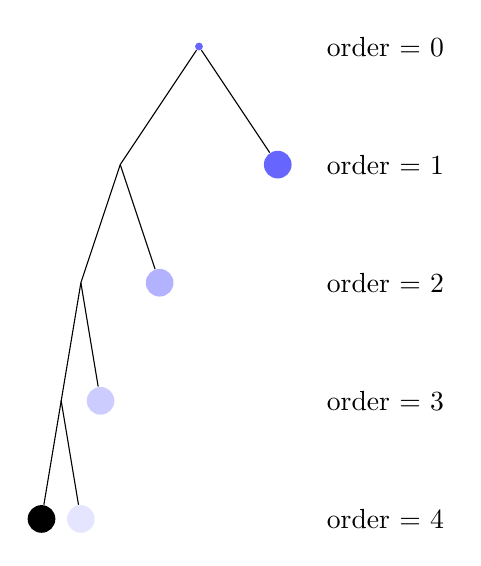
\begin{tikzpicture}
		[
			every node/.style={
					fill=blue!60,circle,inner sep=1pt,minimum width=10pt},
			level 1/.style={sibling distance=20mm,nodes={fill=blue!60}},
			level 2/.style={sibling distance=10mm,nodes={fill=blue!30}},
			level 3/.style={sibling distance=5mm,nodes={fill=blue!20}},
			level 4/.style={sibling distance=5mm,nodes={fill=blue!10}}]
		\node[minimum width=0pt] (Root) {}
		child {
				child {
						child {
								child {node[fill=black]{}}
								child {node{}}
							}
						child {node{}}
					}
				child {node{}}
			}
		child {node{}};
		\begin{scope}[every node/.style={right}]
			\xdef\level{Root}  % Initial top level
			\def\rightmostnode{Root-2}   % Name of the node with greater x coordinate
			\foreach \order in {0,...,4}
				{
					\path (\level -|\rightmostnode)
					++(5mm,0) node {order = \order};
					\xdef\level{\level-1}
				}
		\end{scope}
	\end{tikzpicture}

	\caption{\label{fig:buddy split tree} 伙伴系统分割树型示意图}
\end{figure}

若调用者需要释放之前分配的页面,分配器会找到它的伙伴(见Listing~\ref{lst: find_buddy_pfn}),如果伙伴空闲,
则把要释放的块和它的伙伴合并,并且把该伙伴从空闲列表中删除.
然后继续寻找新合成的块的伙伴,尝试合并,直到伙伴不空闲或没有伙伴,无法合并为止.
最后把合并而来的内存块加入到对应次的空闲列表中.
合并是分割的逆过程,图~\ref{fig:buddy split}和图~\ref{fig:buddy split tree}
在合并伙伴的过程中仍然适用.

伙伴系统可以达到很高的内存利用率,在模拟中可以在无法分配之前达到95\%的利用率.
而且,伙伴系统不仅无需定期的压缩和移动来减少碎片,
出现分割和合并操作的频率也很低,
总体上使用得最频繁的大小的块也是最多的.\cite{taocp1}

\begin{readsrcbox}{Buddy system}
	伙伴系统分配器的实现主要在 \linuxsrc{mm/page_alloc.c} 中.

	各种分配内存的函数最终都会调用 \lstinline{__get_free_pages()} 函数,
	通过向其传递不同的选项(GFP flags)来控制分配器的行为.
	最终进行分配的函数是 \lstinline{rmqueue()}.
	它寻找最小的空闲块,并调用 \lstinline{expand()} 来对较大的空闲块进行分割.

	处理释放工作的是函数 \lstinline{__free_one_page()},
	它负责释放块,合并伙伴,更改空闲队列.
\end{readsrcbox}

\subsection{slab 分配器}
使用伙伴系统的页面分配器是Linux内核的最底层的内存分配系统,
在页面分配器的层次之上,还有更精细的内存分配机制.
Linux内核采用slab分配器来为内核中常用的多种需要动态分配的对象管理内存.
\index{slab allocator}
在slab分配器中,同种对象连续地存储在一起,批量地分配内存,
有状态的对象在释放和分配之间,状态仍缓存在原来的空间中.
批量存储同样的对象有助于提高空间利用率、减小了内碎片化程度,
而状态的缓存则避免了频繁初始化的开销.
\cite{bonwick1994slab}
\begin{qbox}{什么是对象?}
	slab分配器管理的对象可以是存储状态的某种控制块,如进程控制块、inode等.
	也可以是无状态的缓冲区等.\index{kernel object}
\end{qbox}

在slab分配器中,对象存储在cache中,
每种对象都有自己的cache\index{slab allocator!cache},
每一个cache中又有若干slab.\index{slab allocator!slab}
slab是一小段连续的空间,通常为就为一个页面,
要分配的对象就连续地存放在slab中.
slab的分配过程中,内部的所有对象就都完成了初始化,
所以从slab中分配得到的对象永远都是已经初始化的,
调用者在分配和释放的时候既不用重新初始化也不用做全部的清理工作,
清理工作会在整个slab被销毁的时候进行.
这样的设计是考虑到有些对象的初始化开销甚至大于分配内存的开销,
保留共用的初始状态可以显著减少由于反复初始化而带来的性能损失.\cite{bonwick1994slab}

借助slab还可以减少内碎片化程度.
slab根据存储对象的状态被分为三种:
\begin{itemize}
	\item 存满对象的;
	\item 存有对象但没有装满的;
	\item 没有存储对象的,全部空闲的;
\end{itemize}
在分配新的对象时,若有没装满的slab,一定使用没装满的slab,而不引入新的碎片;
只有在没有部分装满的slab时,才会使用空闲的slab或者分配新的slab.

\begin{readsrcbox}{Slab allocator}
	slab分配器的实现在 \linuxsrc{mm/slab.c}.
\end{readsrcbox}

%%% Local Variables:
%%% mode: latex
%%% TeX-master: "linux_zh"
%%% End:
